\documentclass{resume}

\begin{document}

\fontfamily{ppl}\selectfont

\noindent
\begin{tabularx}{\linewidth}{@{}m{0.8\textwidth} m{0.2\textwidth}@{}}
{
    \Large{Foma Shipilov} \newline
    \small{
        \clink{
            \href{mailto:foma@shipilov.ru}{foma@shipilov.ru} \textbf{·} 
            {\fontdimen2\font=0.75ex [removed]} 
            \textbf{·} 
            \href{http://shipilov.ru}{shipilov.ru}
        } \newline
        Moscow, Russia
    }
} & 
{
    \hfill
    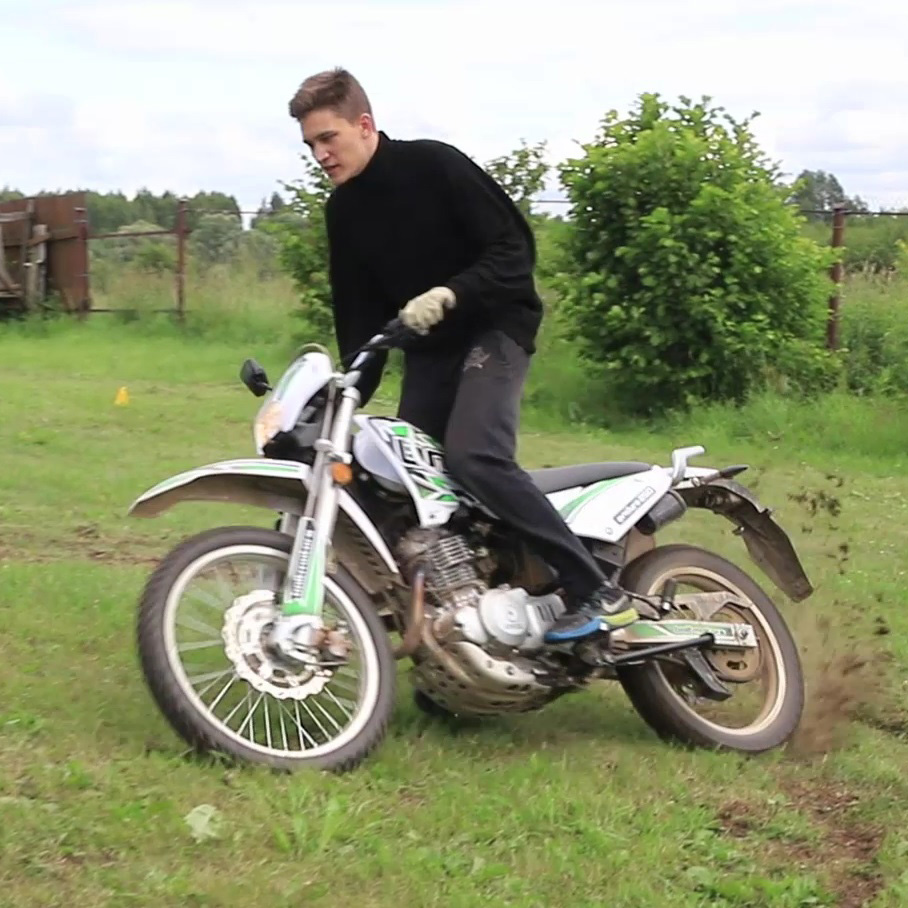
\includegraphics[width=2.8cm]{images/gr.jpg}
}
\end{tabularx}
\begin{center}
\begin{tabularx}{\linewidth}{@{}*{2}{X}@{}}
% left side %
{
    \csection{EXPERIENCE}{\small
        \begin{itemize}
            \item \frcontent{Huawei}{Assistant Engineer -- Noah’s Ark lab\vspace{0.2em}}{-- Remastered TV-series under ``Low-quality movies enhancement using Generative Adversarial Networks'' project;\newline
            -- Developed non-linear convolutional degradation model for super-resolution of real-world images.}{November 2020 -- September 2021}
            \item \frcontent{Higher School of Economics}{Intern-researcher -- Laboratory of Methods for Big Data Analysis (LAMBDA)}{-- Developing surrogate generative models for fast simulation of FARICH detector.}{November 2021 onwards}
        \end{itemize}
    }
    \csection{EDUCATION}{\small
        \begin{itemize}
            \item \frcontent{B.S. Computer Science}{Higher School of Economics}{}{Currently undergoing}
            \item \frcontent{Physics \& Tech class}{Moscow Institute of Physics and Technology, Kurchatov Institute}{}{2019}
            \item \frcontent{Zaochnaya Fiziko-Tekhnicheskaya Shkola}{Moscow Institute of Physics and Technology}{}{2019}
        \end{itemize}
    }
    \csection{PROJECTS}{\small
        \begin{itemize}
            \item \frcontent{RealSR \clink{\href{https://github.com/SergejVolkov/SR_base}{[github.com]}}}{Implementation of RealSR CVPRW 2020 paper}{}{Pytorch}
            \item \frcontent{Visual Turing \clink{\href{https://github.com/SergejVolkov/turing_machine_emulator}{[github.com]}}}{Advanced Turing machine BASH-like IDE}{}{C++}
            \item \frcontent{babelia.meaning \clink{\href{https://github.com/SergejVolkov/babelia.meaning}{[github.com]}}}{}{}{Python, OpenCV}
        \end{itemize}
    }
} 
% end left side %
& 
% right side %
{
    \csection{SKILLS}{\small
        \begin{itemize}
            \item \textbf{Technologies} \newline
            {\footnotesize C, C\#, C++, Python, Pytorch, x86/ARM Assembly, Haskell, GDB, GNU/Linux, Java/Android, HTML5/CSS, JavaScript }{}{}
            \item \textbf{Patterns \& Practices} \newline
            {\footnotesize Deep Learning, Computer Vision, Object Oriented Programming, Physical Simulations}
        \end{itemize}
    }
	\csection{AWARDS \& RECOGNITION}{\small
		\begin{itemize}
			\item \frcontent{``Vysshaya Liga'' Math \& Informatics}{Higher School of Economics}{Degree I \& III Diploma}{2021 {\textnormal\&} 2022}
			\item \frcontent{``Ya Professional'' Math Olympiad}{Yandex}{Prize-winner}{2021, 2022}
			\item \frcontent{``Pokori Vorob'yovi Gori'' Math Olympiad}{Moscow State University}{Winner}{2019}
			\item \frcontent{``Phystech'' Math \& Physics Olympiads}{Moscow Institute of Physics and Technology}{Winner}{2019}
		\end{itemize}
	}
    \csection{OTHER HIGHLIGHTS}{\small
        \begin{itemize}
            \item {\footnotesize Conducted biology studies within \textit{Structural and Functional Research of G-protein-coupled Cell Surface Receptors Using 3D Modeling} school project.}
        \end{itemize}
    }
    \csection{HOBBIES \& INTERESTS}{\small
        \vspace{0.32cm}
        \begin{tabularx}{\linewidth}{@{}*{4}{>{\centering\arraybackslash}X}@{}}
            {\centering
            
\includegraphics[width=0.8cm]{images/animation.png}
            } &
            {\centering
            
\includegraphics[width=0.8cm]{images/music.png}
            } & 
            {\centering
            
\includegraphics[width=0.8cm]{images/physics.png}
            } &
            {\centering
            
\includegraphics[width=0.8cm]{images/probability.png}
            } \\
            {\footnotesize Animation} & {\footnotesize Composing} & {\footnotesize Physics} & {\footnotesize Probability Theory}
        \end{tabularx}
    }
}
\end{tabularx}
\end{center}
\end{document}
